\documentclass[runningheads]{llncs}
%
\usepackage[T1]{fontenc}
\usepackage{hyperref}
\usepackage{graphicx}
\usepackage{tikz}
\usepackage{wrapfig}
\usepackage{package/mathpartir}
\usepackage{todonotes}
\usepackage{xspace}

\usepackage{package/regles}
\usepackage{mathtools}
\usepackage{ amssymb }

\usepackage{minted}

\usepackage{caption}
\usepackage{subcaption}

\usepackage{package/formal-grammar}

\newcommand{\ruleFmt}[1]{\textsc{(#1)}}
\newcommand{\ruleDef}[1]{\hypertarget{#1}{\ruleFmt{#1}}}
\newcommand{\ruleRef}[1]{\hyperlink{#1}{\ruleFmt{#1}}}

\newcommand{\Nat}{{\mbox{$\mathbb{N}$}}}
\newcommand{\tuple}[1]{\ensuremath{\langle #1\rangle}}

\newcommand{\directions}{\dirFmt{\mathsf{D}}}
\newcommand{\internalState}{{\mathcal{I}}}

% Je suis assez d'avis de distinguer la direction des blocks et des trains
\newcommand{\forward}{\ensuremath{\mathtt{f}}}
\newcommand{\backward}{\ensuremath{\mathtt{b}}\xspace}
\newcommand{\sucblock}{{\mathtt{suc}}}
\newcommand{\throughS}{{\mathtt{through}}}

%% Modèle
\newcommand{\modelSet}{\ensuremath{\mathbb{M}}}

%% Train directions
\definecolor{dircolor}{rgb}{1.0, 0.13, 0.32}
\newcommand{\dirFmt}[1]{{\color{dircolor} #1}}
\newcommand{\dirForward}{\ensuremath{\dirFmt{\forward}}\xspace}
\newcommand{\dirBackward}{\ensuremath{\dirFmt{\backward}}\xspace}
\newcommand{\dirStop}{\ensuremath{\dirFmt{\star}}\xspace}

%% Positions
\definecolor{poscolor}{rgb}{0.6, 0.45, 0.32}
\newcommand{\posFmt}[1]{{\color{poscolor}{#1}}}
\newcommand{\blocks}{{\posFmt{\mathsf{B}}}}
\newcommand{\bid}[1]{\ensuremath{\posFmt{b_{#1}}}}
\newcommand{\suc}[3]{\ensuremath{\sucblock(\posFmt{#1}, \dirFmt{#2}, \swFmt{#3})}}

%% Switches
\definecolor{swcolor}{rgb}{0.4, 0.23, 0.56}
\newcommand{\swFmt}[1]{{\color{swcolor}{#1}}}
\newcommand{\sid}[1]{\ensuremath{\swFmt{s_{#1}}}}
\newcommand{\turnouts}{\swFmt{\mathsf{\Theta}}}
\newcommand{\switches}{\ensuremath{\swFmt{\sigma}}}
\newcommand{\networkConf}{\ensuremath{\swFmt{\Sigma}}}
\newcommand{\nosuc}{\ensuremath{\swFmt{\bot}}}
\newcommand{\updateSwitch}[3]{\ensuremath{#1[\swFmt{#2}\leftarrow #3]}}

%% Trains
\definecolor{traincolor}{rgb}{0.2, 0.2, 0.6}
\newcommand{\trainFmt}[1]{{\color{traincolor} #1}}
\newcommand{\trainTuple}[4]{\langle \trainFmt{#1}, \posFmt{#2}, \dirFmt{#3}, #4 \rangle}
\newcommand{\trainSeq}{\ensuremath{\trainFmt{\Gamma}}\xspace}
\newcommand{\trains}{{\trainFmt{\mathsf{T}}}}
\newcommand{\tid}[1]{\ensuremath{\trainFmt{t_{#1}}}}

%% Train program
\newcommand{\su}[2]{{\mbox{$\mathtt{startuntil}(\dirFmt{#1}, \posFmt{#2})$}}\xspace}
\newcommand{\trainConcat}[2]{#1 \cdot #2}
\newcommand{\emptyTrainProg}{\varepsilon}

%% Regulator
\newcommand{\handlerOf}[2]{\ensuremath{#1[\trainFmt{#2}]}}
\newcommand{\popHandlerHead}[2]{\ensuremath{{\tt pop}(#1[\trainFmt{#2}])}}
\newcommand{\substHandlerHead}[3]{\ensuremath{#1[\trainFmt{#2} \leftarrow #3]}}
\newcommand{\actionsOf}[1]{\ensuremath{#1.{\tt act}}}
\newcommand{\blockOf}[1]{\ensuremath{#1.{\tt block}}}
\newcommand{\handler}[2]{\tuple{#1, #2}}
\newcommand{\nextAct}[1]{\ensuremath{#1.{\tt cont}}}

%% Regulator's Program
\newcommand{\regTuple}[3]{\tuple{#1, #2, #3}}
\newcommand{\evGuard}[2]{\ensuremath{\mathtt{ev}(\trainFmt{#1}, #2)}}
\newcommand{\ev}[3]{\evGuard{#1}{#2}: #3}
\newcommand{\incr}[1]{{\mbox{\ensuremath{\mathtt{incr}(\posFmt{#1})}}}\xspace}
\newcommand{\turn}[2]{{\mbox{\ensuremath{\mathtt{turn}(#1, #2)}}}\xspace}
\newcommand{\auth}{{\mbox{\ensuremath{\mathtt{auth}}}}\xspace}
\newcommand{\tokens}{\ensuremath{T}}
\newcommand{\tokenOf}[1]{\ensuremath{T(\posFmt{#1})}}
\newcommand{\regulator}{\ensuremath{R}}
\newcommand{\wait}[2]{{\mbox{\ensuremath{\mathtt{wait}(\posFmt{#1}, #2)}}}\xspace}
\newcommand{\regConcat}[2]{#1 \cdot #2}
\newcommand{\incrToken}[2]{\ensuremath{#1. {\tt incr}(\posFmt{#2})}}

%% Intial actions & event.
\newcommand{\initialHandler}[1]{\handlerOf{#1}{\star}}
\newcommand{\sendred}[2]{\ensuremath{{\tt sendred}(#1, #2)}}

%% Sequences
\newcommand{\push}[2]{\ensuremath{\mathtt{push}(#1, #2)}}
\newcommand{\pop}[1]{\ensuremath{\mathtt{pop}(#1)}}

%% Signals
\newcommand{\sigred}{{\mbox{${\color{red!50!black}\mathtt{r}}$}}\xspace}
\newcommand{\siggreen}{{\mbox{${\color{green!50!black}\mathtt{g}}$}}\xspace}
\newcommand{\deviate}{{\mbox{$\mathtt{v}$}}\xspace}
\newcommand{\direct}{{\mbox{$\mathtt{d}$}}\xspace}
\newcommand{\signalF}[2]{\ensuremath{\signals(\posFmt{#1}, \dirFmt{#2})}}
\newcommand{\signals}{\ensuremath{F}}
\newcommand{\setSignalsTo}[2]{\signals.{\tt set\_to}(#1, #2)}
\newcommand{\updateSfty}[4]{{\tt updateSfty}(\signals, #1, #2, #3, #4)}
\newcommand{\updateSignal}[4]{\ensuremath{#1[\tuple{\swFmt{#2}, \dirFmt{#3}}\leftarrow #4]}}

%% State
\newcommand{\stateTuple}[4]{\tuple{#1, #2, #3, #4}}

%% Guard
\definecolor{guardcolor}{rgb}{0.53, 0.66, 0.42}
\newcommand{\guardFmt}[1]{{\color{guardcolor} \ensuremath{\mathtt{#1}}}}
\newcommand{\guardT}{\guardFmt{T}}
\newcommand{\guardS}{\guardFmt{S}}
\newcommand{\guardR}{\guardFmt{R}}
\newcommand{\guardG}{\guardFmt{G}}
\newcommand{\guardI}{\guardFmt{I}}
%% Buffer
\newcommand{\bufferFmt}[1]{#1}
\newcommand{\head}[1]{\ensuremath{{\tt hd}(#1)}}
\newcommand{\buflen}[1]{\ensuremath{{\tt len}(\bufferFmt{#1})}}
\newcommand{\bufhead}[1]{\head{\bufferFmt{#1}}}
\newcommand{\buftail}[1]{\ensuremath{{\tt tl}(\bufferFmt{#1})}}
\newcommand{\emptyList}{\ensuremath{\varepsilon}}
\newcommand{\bufTrainSet}{\ensuremath{\bufferFmt{\mathbb{B}_t}}\xspace}
\newcommand{\bufSigSet}{\ensuremath{\bufferFmt{\mathbb{B}_s}}\xspace}
\newcommand{\bufTrain}{\ensuremath{\bufferFmt{B_t}}\xspace}
\newcommand{\bufSig}{\ensuremath{\bufferFmt{B_s}}\xspace}


%% Reduction relation
\newcommand{\reduces}{\ensuremath{\rightarrow}}
\newcommand{\redTuple}[4]{\ensuremath{\tuple{#1, \bufferFmt{#2}, \bufferFmt{#3}, #4}}}

%% Rule predicates
\newcommand{\requestS}[3]{\ensuremath{{\tt RequestS}(\trainFmt{#1}, \posFmt{#2}, #3)}}
\newcommand{\nextWait}[1]{\ensuremath{{\tt NextWait}(#1)}}




\begin{document}
%
\title{Formal verification of train route planning}
%
%\titlerunning{Abbreviated paper title}
% If the paper title is too long for the running head, you can set
% an abbreviated paper title here
%
\author{Lucas Villaume \and Guillaume Bonfante \and Martin Vassor}
%
\authorrunning{L. Villaume et al.}
% First names are abbreviated in the running head.
% If there are more than two authors, 'et al.' is used.
%
\institute{Université de Lorraine, CNRS, Inria, LORIA, F-54000 Nancy, France}
%
\maketitle
%
\begin{abstract}
	% Contexte
	Trains networks are critical system which failure may lead to numerous fatalities, in case of crashes, or important loss, if trains are not properly routed. 
	% Problème
	In this paper, our goal is to formally verify the correctness of train routes. More precisely, we verify the absence of deadlocks, the termination, and the absence of crashes.
	% Approche
	To address this question, we model train systems on paper and in TLA+. Our model includes trains, as well as switches, detection sensors and traffic lights. Both switches and traffic lights are controlled by a regulator upon train events. We provide trains and the regulator with orders, characterising the schedule, which is then checked using TLA+'s model checker.
	% Resultats
	Our contributions are threefold: first, we provide formal model of railroad networks and schedules; second, we implement this model as a TLA+ specification and we report tests on checking schedules on a non-trivial network, composed of 3 trains, 8 blocks and 5 switches; finally we show how to sequentially compose schedules, which we check against our TLA+ specification.

\keywords{Train routing \and Model checking \and Formal methods \and TLA+}
\end{abstract}


\section{Introduction}
\label{sec:introduction}

This contribution finds its origin in a cyber-warefare we are organising for students at the University of Lorraine concerned by cyber-security, see~\cite{CHE}. In the game-play, we have both IT infrastructures and physical systems, with connections between them. On the physical side, we built a small train network that tries to be a good model of real systems.  Our system manages customer informations, train regulation and finally the physical/infrastructure layer. Attackers can hit any of the three parts: disfiguring the website, changing a platform or blocking a signal. Defenders will protect their system, typically via a strict network policy.




\paragraph{Routing trains.}
\todo{Ajouter: tout est automatique}
Routes are computed on the fly. The schedule is renewed every "day"\footnote{We use a time scale factor: one of our "day" corresponds to 20 minutes in real time.}  and we introduce some randomness in the process: beyond some routine daily planning, some trains are inserted/deleted, some trains departure/destination may change, and so on. We simulate also delays. Finally, in our model, we distinguish freight and  passengers routes giving priority to the latter. Routes are recomputed each time a train has finished its duty. The general motivation of this paper is to propose a lightweight scheduling solution that is adapted to the fully automatic control, that takes into account the distributed nature of the system, that is reliable and does not suffer from interlocking.  
 
We can now describe in more detail the working assumptions we are making about planning.  First, we have sensors on the rails at the two ends of each block. Accordingly,  we can catch train entrances within blocks. We make the hypothesis that this task is performed without errors. Second, the switches can be swapped from one position to the other, again, we suppose it is done without fault. Our method could cope such issues, but we leave that for future work. 
 
  Third, for trains, we have a simple policy.  According to its plan, a train may start in some direction (Forward/Backward) up to some final position. Then, once started, the train will run according to the signals: when green, it (re-)starts, when red, it stops.  We do not make hypotheses on the durations of travels, but once a train is running, it will reach in finite time the next block. Trains run in parallel independently. One train may enter a block, while an other is crossing some switch and the third one is breaking. There is no communications between the trains.

Fourth,  the regulator is capable of reading train block entrance events, requiring some switch swap and finally locking (that is make sure a signal is red)/unlocking some signal. We consider that those latter operations can be carried out without delay. Finally, the regulator may append some new duty to a train. To sum up, to control the train mouvements, the regulator can only lock/unlock signals. Naturally, a signal intended to block train $T_1$ may block $T_2$ if not set at the right time.   
 
 Parler de la stratégie, du modèle générale. All these operations are done by what we call  \emph{orders}. Roughly speaking, trains Orders have the shape "Start in direction Until position". Regulator orders are: \todo{en parler}. 
 
 
 To sum up, the regulation policy can be seen as an asynchronous distributed system. The N trains and the regulator are independent agents. That led us to TLA+, a framework introduced by Leslie Lamport for these kind of problems~\cite{Lamport}.  
 
\todo{ Comparaison avec les travaux antérieurs / lit review}
 
 
Due to the distributed nature of the regulation, building a safe policy can be very tricky. We want to show in this paper that tools from formal methods are very useful in this respect.  In this paper, we describe in  a first step the formalisation process. We go up to a TLA+ specification that will allow us checking two properties of route orchestration: safety and liveness. This is our first research question. 

Our second research question is the related to the following need. Suppose we want to append a new duty once a train reached its destination. This can be formalised as a composition problem (how to compose/concatenate some routes with some others). We describe such a composition procedure and then, again, we check that the routes are both safe and deadlock free. 

For our last research problem, we show that TLA+ may be used to refine a regulation policy. In our first attempts, we had typically some deadlocks issues. We have been able to detect them via TLA+ and then to provide some correction. 

\paragraph{Motivation.}

Over the last decades, we observe a general and increasing interest of formal methods for verification and validation of safety-critical systems, including railway networks.
In \cite{Ferrari_Formal_2022}, Ferrari et al. present a survey of use cases of formal methods in railways development. They identify various phases of development phases where formal methods have been used, ranging from planning to maintenance via implementation, testing, etc., as well as most frequently studied subsystems (interlocking systems being the most formally verified component). In this paper, focus specifically on train \emph{routing}, i.e. finding correct train schedules (for some correctness criteria). This topic is related to that of interlocking (we prevent trains from using simultaneously some elements), but from the viewpoint of trains and their routes, while the viewpoint of interlocking is mostly trackworks.

In~\cite{lusby_railway_2011}, Lusby et al.\ survey works on train routing. In this context, we can distinguish two problems: automated routing and routing verification. The former deals with automatically finding train routes satisfying some properties. Lusby et al.\ mention that solving this problem, in highly interconnected network, is not feasible in practice. In this paper, we address the second problem: verifying whether a train routing satisfies correctness criteria (without considering how it is obtained). In particular, we are interested in formal verification of such routings.

\begin{wrapfigure}[10]{r}{0.28\textwidth}
	\begin{minipage}{0.28\textwidth}
		\centering
		\vspace{-8mm}
		\includegraphics[height=30mm]{maquette.png}
		\caption{The model.}
		\label{fig:maquette}
	\end{minipage}
\end{wrapfigure}

\paragraph{Model.}
Before delving further in the details, we introduce a real-world N-scale train model (\ref{fig:maquette}), which shaped our approach and was used to test our results. This model has 8 blocks, 5 switches. Each block is bidirectional with a signal at each end. Blocks size goes from 25cm to 70cm. We operate three trains concurrently. Due to the size of the model, we reduced our signals  to "red" and "green" status, the trains being too close to each other for a finer modelling of signals. Furthermore, in case of a red signal, we make the hypothesis that the train are able to stop before reaching the end of the block.

\begin{wrapfigure}[8]{r}{0.45\textwidth}
	\vspace{-6mm}
	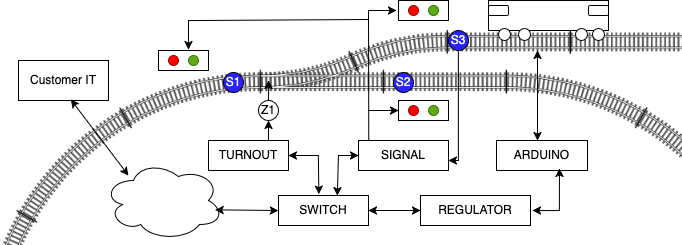
\includegraphics[height=20mm]{TrainSchema.png}
	\caption{The computer infrastructure.}
	\label{fig:computers}
\end{wrapfigure}

Switches and signals are controlled by two Raspberry-pi computers, which communicate so that signals are safe w.r.t. switches. A third computer, called the \emph{regulator}, manages the traffic. It can request switches updates, lock signals\footnote{The regulator can explicitly request a green signal to turn red, for traffic control. However, if the signal controller requires a signal to be red, for safety reasons, the regulator can not force it green.}, and route trains. To control trains, an Arduino board is used and simulates train drivers. The Arduino board communicates with the regulator to query states of signals, which would be seen by the driver in real life (see Fig. \ref{fig:computers}). 

\paragraph{Contributions.}
Our main contributions are:
\begin{itemize}
	\item Building a formal model of train network. Contrary to most existing works, our model makes very few assumptions: tracks are not directed, we do not distinguish between tracks and stations (platforms are regular tracks).
	\item Writing the TLA+ specification of our model. This specification allows to model check routings.
	\item Defining a composition operator, allowing to build up large routes from smaller part. We use TLA+ to model check resulting composed routes.
\end{itemize}

\paragraph{Related works.}


\paragraph{Outline.}
In Section~\ref{sec:model_configurations}, we introduce the main building blocks of our model: network infrastructure, trains and the regulator. In Section~\ref{sec:model_semantics}, we present the dynamic aspects of our system: how trains can move and how the regulator schedules them. We conclude this section by stating what we expect of correct networks. Then, in Section~\ref{sec:tla-formalisation}, we present a TLA+ implementation of our model, which we use to check network correctness: model checking a schedule \emph{certifies} its correctness. Our last contribution, in Section~\ref{sec:composition}, explains how to build large schedules by composing smaller ones. While we don't prove the correctness \emph{by construction} of composed schedules, we use the TLA+ implementation to certify, \emph{a posteriori}, the correctness of composed schedules.

% ############################# %
% Espace réservé aux encadrants %
% ############################# %


\paragraph{Notations.}

Given some set $S$ and some $x \not\in S$, we denote by $S_x = S \cup \{ x\}$.  An other notation: given some function $f: X \to Y$, $x \in X$ and $y \in Y$, we denote by $f[x \leftarrow y]$, the function:
 $$f[x \leftarrow y] \triangleq \left\{  \begin{array}{ll} x &\mapsto y\\
x' \neq x \in X &\mapsto f(x')
\end{array}\right.$$


\section{Model configurations}
\label{sec:model_configurations}

In this section, we present configurations of our model, i.e. how we represent, at a given point in time, the state of our network. The dynamic rules of train routing are then presented in the following section.

Our model is has $k+1$ agents corresponding to the $k$ trains and the Regulator. Those agents take place on an infrastructure consisting of a track network equipped with signals. We first present the infrastructure model, then the agents.

\subsection{Infrastructure}

\paragraph{The network.} 

We suppose that the train network can be described as follows. First, we consider a set of $n$ blocks: $\blocks = \{ \bid{1}, \bid{2}, \ldots, \bid{n}\}$. Blocks are oriented: there is a $\dirForward$ (forward) end and a $\dirBackward$ (backward) one. Let $\directions = \{\dirForward, \dirBackward\}$ be the set of directions.  Second, we consider a set of $m$ trackworks\footnote{For the sake of simplicity, in this paper, we only consider switches. Our work can easily be extended to crossings and double slip switches (e.g. crossings have only one internal state and double slip switches have four states).}: $\turnouts = \{\sid{1}, \ldots, \sid{m}\}$. Trackworks are characterized by an internal state: switches can be in direct or deviate position (next denoted '\direct' and '\deviate'). Let $\internalState$ denotes the set of internal states. A \emph{network configuration} is given by a function $\sigma: \turnouts \to \internalState$. Let $\networkConf$ denotes the set of all network configurations. For instance, for two turnouts $\theta = \{\sid{1}, \sid{2}\}$, the function $\sid{1} \mapsto \deviate, \sid{2} \mapsto \direct$ states that switch $\sid{1}$ is in deviate position while \sid{2} is in direct one. The latter function is also described via an array  $[\deviate, \direct]$ giving states in trackwork order.

The network is then described as a triple $(\blocks, \turnouts, \sucblock)$ where $\sucblock$ is a partial function indicating the following block given a starting position, a direction and a network configuration: $\sucblock: \blocks\times \directions \times \networkConf \to \blocks$. We note $\suc{\bid{id}}{d}{\switches} = \nosuc$ when it is undefined. From an abstract point of view, the topology of the network reduces to that data.  


\paragraph{Signals.}
\todo{Est-ce qu'on met les signaux dans les agents ?}
At each end of the blocks, there is a signal whose state is \sigred (red) or \siggreen (green). In other words, the status of signals is described by a function $\signals: \blocks \times \directions \to \{ \sigred, \siggreen\}$. The signal status is determined by the network configuration and explicit locking requests. Given some signal status $\signals$, a block $\bid{id}$ and a direction $\dirFmt{d}$, $\signalF{\bid{id}}{d} = \sigred$ means the signal guarding the exit of block $\bid{id}$ in direction $\dirFmt{d}$ is red, and we expect trains not leaving that block going in this direction\footnote{Our semantics, presented in Section~\ref{sec:model_semantics}, ensure such behaviour.}. We note $\setSignalsTo{\bid{\text{tgt}}}{c}$ the signal state $\signals$ except signals of block \bid{\text{tgt}}, which are turned to color $c$: 
$$(\setSignalsTo{\bid{\text{tgt}}}{c})(\bid{\text{from}}, \dirFmt{d}) = \begin{cases}
	c & \text{if }\bid{\text{from}} = \bid{\text{tgt}}\\
	\signalF{\bid{\text{from}}}{d} & \text{otherwise}
\end{cases}$$


\subsection{Agents}
\paragraph{Trains.}
We now present the train model. We consider a set of $k$ trains. 
Each train is characterised by an identifier, a position, a direction, and a list of orders.
\begin{itemize}
	\item Train identifiers form a set  $\trains = \{\tid{1}, \ldots, \tid{k}\}$, each train having its own identifier.
	\item The position is the index of the block currently occupied by the train.
	\item The direction (taken from $\directions_\dirStop = \{\dirBackward, \dirForward, \dirStop\}$) indicates the direction the train is ordered to go towards, where \dirStop indicates the train has no direction order at the moment. The direction represents the current move order, but does not mean the train is actually moving: it can be blocked at a signal.
	\item Orders are a (possibly empty) sequence of orders $\su{d}{\bid{1}\dots\bid{n}}$ ($\dirFmt{d} \in \directions$, $\bid{i} \in \blocks^\star$). Such order states that the train direction is set to $\dirFmt{d}$ and that the train will use blocks $\bid{1}\dots\bid{n}$. An empty sequence is denoted $\emptyTrainProg$. We intend successive \su{d_i}{...} orders of the list to alternate directions \dirForward{} and \dirBackward{}. Two successive orders with the same direction can easily be merged into a single one.
\end{itemize}

Thus, each train is a quadruple $\trainFmt{t} = \trainTuple{\tid{id}}{\bid{id}}{d}{P}$ with $\tid{id}$ the train's identifier, $\bid{id}$ its position, $\dirFmt{d}$ its direction and $P$ its sequence of orders. Trains are collected in a sequence $\trainSeq = (\trainFmt{t_1}, \ldots, \trainFmt{t_k})$ where each $\trainFmt{t_i}$ being the tuple of train $\trainFmt{i}$. 


\paragraph{The Regulator.}
The regulator is in charge of the execution of the routing.
It is characterised by a routing program, a token list, and a waiting set.

\begin{itemize}
	\item The routing program $E$ specifies how the regulator should react to events (i.e. when a train enters a block). A program is a collection of rules to apply upon each event (called an \emph{event handler}). We detail further event handlers below.
	\item The token list, denoted $\tokens$, is a function  $\tokens: \blocks \to \Nat$ associating a token level to each block. Those tokens are used to prevent multiple trains accessing the same block at the same time.
	\item The waiting set is a set $W \subseteq \blocks \times \blocks \times \Nat \times \trains$. A 4-tuple $\tuple{\bid{src}, \bid{dst}, n, \tid{id}} \in W$ means that train \tid{id} is currently waiting in the block \bid{src} for $\tokenOf{\bid{dst}}$ to be increased up to $n$.
\end{itemize}

Overall, the regulator is a tuple $R = \regTuple{E}{\tokens}{W}$. We note $\incrToken{T}{\bid{id}}$ the list of tokens identical to $T$, except for $\tokenOf{\bid{id}}$, which is incremented.

\paragraph{Regulator's event handlers.}

Train events are handled by the regulator. Upon such events, the regulator can take actions such as turning a switch, allowing or blocking a train, etc.. The regulator is equipped with a routing program. This routing program contains, for each train, a list of handlers. A handler is a tuple $\tuple{\bid{id}, A}$, where $\bid{id}$ is the position the train occupies when triggering the event, and $A$ is the list of orders associated with that event. For a given train, the first handler of the list is the set of actions that have to be executed on the train's first event, second handler for the second event, and so on.
Given a routing program $E$, we note $\handlerOf{E}{\tid{id}}$ the list of handlers of train $\tid{id}$, $\head{\handlerOf{E}{\tid{id}}} = \handlerOf{E}{\tid{id}}[1]$ the first handler of the list. Given a handler $h = \tuple{\bid{id}, A}$, we note $\actionsOf{h}$ (resp. \blockOf{h}) the list of action (resp. the block id) of $h$. We note $\nextAct{\handlerOf{E}{\tid{id}}}$ the routing program $E$ where the first event handler of train $\tid{id}$ is replaced with $\handler{\blockOf{\head{\handlerOf{E}{\tid{id}}}}}{\buftail{\actionsOf{\head{\handlerOf{E}{\tid{id}}}}}}$, i.e. where the first action of the first handler of train \tid{id} is removed. We note $\popHandlerHead{E}{\tid{id}}$ the routing program $E$ where the first event handler of train \tid{id} is removed, i.e. where $\handlerOf{E}{\tid{id}}$ is replaced by $\buftail{\handlerOf{E}{\tid{id}}}$.

Actions contained in a handler are of the four following kinds:
\begin{description}
	\item [\wait{\bid{id}}{n}:] the train waits until the token of block \bid{id} reaches value $n$
	\item [\incr{\bid{id}}:] this increments the token $\bid{id}$ in $T$, thus releasing a train waiting
	\item [\turn{\sid{id}}{s}:] this turns the switch $\sid{id}$ into the $s$ state: $\sigma\cdot\turn{\sid{id}}{s} = \sigma[\sid{id} \leftarrow s]$
	\item [\auth:] a shortcut for waiting on oneself
\end{description}

\paragraph{Model.}
Overall, states of our model are tuples $\tuple{\trainSeq, \regulator, \switches, \signals}$ where $\trainSeq$ is a set of train tuples, $\regulator$ a regulator tuple, $\switches$ a network configuration (indicating trackworks states) and $\signals$ a signals state function. We suppose all train tuples in $\trainSeq$ have a different identifier. Notice that $\sucblock$ is not part of the state. Instead, the dynamics of the model (see below) is parameterised by $\sucblock$. Let $\modelSet$ be the set of all model states.

\paragraph{Network hypothesis, events, and conventions.}
On the tracks, we suppose there are sensors to detect the presence of trains. More precisely, we suppose that ---by means of the sensors--- the position of every train is known at any time. A \emph{position event} is when a train move from one block to an other one. 

Train speed are not modeled, and we consider trains can always stop within their current block if they have to (e.g. if there outgoing signal of a block is \sigred, we assume the train can stop in time).


\section{Model Semantics/Model dynamics}
\label{sec:model_semantics}

In the previous section, we introduced our model. In this section, we present the dynamics of our model, that is the rules that govern how our model can switch from one state to the other.
We enrich our model with two elements: a guard, which goal is to schedule agents (for instance, it ensures the regulator acts atomically); and a communication buffer, which stores pending events until the regulator treats them. We present those two new elements in the first subsection.
The dynamics is described by means of a reduction relation, characterising the successive states of our model. We define this reduction relation using inference rules in the second subsection.

\todo{Expliquer le temps discret et le mix grand pas/petit pas.}

\subsection{Scheduling and communications}

In our dynamic rules, we distinguish three kinds of rules: one kind for trains, one kind for the regulator, and one kind for updating signals. We intend the signals' and regulator's reactions to be executed atomically. On the other hand, trains evolve much slower. To reflect this behaviour in our rules, we introduce a \emph{guard}. While, in our rules, the reaction of the regulator can take several steps, to implement atomic reaction, the guard blocks the rest of the system. Similarly, upon any train movement or regulator reaction, signals can be updated. In practice, such update happens instantly. To mimick this reaction of signal w.r.t. other events, the guard is in charge of blocking the system until signals are up-to-date.

Essentially, this guard is the state machine shown in Figure~\ref{fig:state_machine_guard}. The four states of the guard are \guardR, \guardS, and \guardT.

\begin{figure}
	\centering
	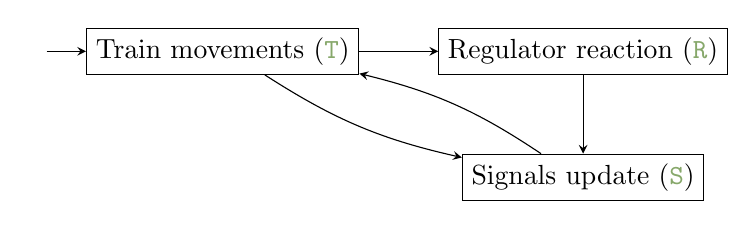
\begin{tikzpicture}
		\node[draw] (trains) {Train movements (\guardT)};
		\node[left=.5cm of trains.west] (zero) {};
		\node[draw, right=of trains] (regulator) {Regulator reaction (\guardR)};
		\node[draw, below=of regulator] (signals) {Signals update (\guardS)};
		
		\draw[-stealth] (zero) to (trains);
		\draw[-stealth] (trains) to[bend right=10] (signals);
		\draw[-stealth] (signals) to[bend right=10] (trains);
		\draw[-stealth] (trains) to (regulator);
		\draw[-stealth] (regulator) to (signals);
	\end{tikzpicture}
	\caption{State machine of the guard.}
	\label{fig:state_machine_guard}
\end{figure}

In our model, a train event represents a train going from one block to another. Train events are not dealt with instantly by the regulator (e.g. two train events can happen before the regulator begins to react to the first one). To characterise this behaviour, train events are stored in a buffer until the regulator uses them. When such thing happens, the train sends a message with its identifier to the regulator. A \emph{train buffer} \bufTrain is a sequence of such events, i.e. of train identifiers.
Similarly, the regulator communicates with signals with a \emph{signal buffer} \bufSig, which is a list of tuples $\tuple{\bid{id}, c}$, indicating that both signals of block $\bid{id}$ should be turned to value $c$. Let \bufTrainSet (resp. \bufSigSet) denote the set of train (resp. signal) buffers.

\subsection{Reduction rules}

States of the system are 4-tuples from $\{\guardR, \guardS, \guardT\} \times \bufTrainSet \times \bufSigSet \times \modelSet$. Our reduction relation is a binary relation on system states, noted $\reduces$: $S_1 \reduces S_2$ means that state $S_1$ can change to $S_2$ (note that this relation is not a function: $S_1$ can reduce to multiple states, due to non-determinism). We define $\reduces$ as the least relation induced by the inference rules presented hereafter.

\paragraph{Train rules.}
We now focus on rules that affect trains. The first rule is \ruleRef{Start}, which is used to change the direction of a train (e.g. to go from a stop to a given direction, or to change direction if the train has to backtrack). This rule can be triggered when the program of the train begins by \su{d^\prime}{N}. This order says that the train should got in direction $\dirFmt{d^\prime}$, and on that direction, it is expected to meet the sequence of block which ids are in $\posFmt{N}$.

\begin{mathpar}
	\inferrule*[left=\ruleDef{Start}]{
		\dirFmt{d} \neq \dirFmt{d^\prime} \and P = \trainConcat{\su{d^\prime}{\posFmt{N}}}{P^\prime}
	}{
		\hspace{3mm} \redTuple{\guardT}{\bufTrain}{\bufSig}{\stateTuple{\trainSeq{}\cup\{\trainTuple{\tid{id}}{\bid{id}}{d}{P}\}}{\regulator}{\switches}{\signals}} \\
		\reduces
		\redTuple{\guardT}{\push{\bufTrain}{\tid{id}}}{\bufSig}{\stateTuple{\trainSeq{}\cup\{\trainTuple{\tid{id}}{\bid{id}}{d^\prime}{P}\}}{\regulator}{\switches}{\signals}}
	}
\end{mathpar}

Conversely, if the train program is empty (i.e. upon termination), the train stops using rule \ruleRef{Stop}.
\begin{mathpar}
	\inferrule*[left=\ruleDef{Stop}]{
		\dirFmt{d} \neq \dirStop
	}{
	\hspace{4mm}  \redTuple{\guardT}{\bufTrain}{\bufSig}{\stateTuple{\trainSeq{}\cup\{\trainTuple{\tid{id}}{\bid{id}}{d}{\emptyTrainProg}\}}{\regulator}{\switches}{\signals}} \\
	\reduces
	\redTuple{\guardT}{\push{\bufTrain}{\tid{id}}}{\bufSig}{\stateTuple{\trainSeq{}\cup\{\trainTuple{\tid{id}}{\bid{id}}{\dirStop}{\emptyTrainProg}\}}{\regulator}{\switches}{\signals}}
	}
\end{mathpar}

The last two rules for trains describe what happens when a train actually moves, i.e. when its position changes. Two cases can occur, depending on the list of intermediate blocks $\posFmt{N}$ in the current order of the train
If $\posFmt{N}$ contains only the upcoming block, then upon leaving the block, the order is removed (rule \ruleRef{UntilNext}); otherwise the upcoming block is simply popped from $\posFmt{N}$ (rule \ruleRef{Until}). Notice that in both cases, the state of the guard changes to \guardS, meaning that signals will be updated immediately after that rule. Finally, when the train reaches intermediate positions (rule \ruleRef{Until}), a train event is enqueued for the regulator.

\begin{mathpar}
	\inferrule*[left=\ruleDef{Until}] {
		\suc{\bid{id}}{d}{\switches} = \bid{id^\prime} \neq \nosuc
		\and
		\signalF{\bid{id}}{d} = \siggreen
		\and
		\posFmt{N}\neq \varepsilon
	}{
		\redTuple{\guardT}{\bufTrain}{\bufSig}{\stateTuple{\trainSeq{}\cup\{\trainTuple{\tid{id}}{\bid{id}}{d}{\trainConcat{\su{d}{[\bid{id^\prime}; \posFmt{N}]}}{P}}\}}{\regulator}{\switches}{\signals}} \\
		\reduces		
		\redTuple{\guardS}{\push{\bufTrain}{\tid{id}}}{\bufSig}{\stateTuple{\trainSeq{}\cup\{\trainTuple{\tid{id}}{\bid{id^\prime}}{d}{\trainConcat{\su{d}{[\posFmt{N}]}}{P}}\}}{\regulator}{\switches}{\signals}}
	}
\end{mathpar}

\begin{mathpar}
	\inferrule*[left=\ruleDef{UntilNext}] {
		\suc{\bid{id}}{d}{\switches} = \bid{id^\prime} \neq \nosuc
		\and
		\signalF{\bid{id}}{d} = \siggreen
	}{
		\redTuple{\guardT}{\bufTrain}{\bufSig}{\stateTuple{\trainSeq{}\cup\{\trainTuple{\tid{id}}{\bid{id}}{d}{\trainConcat{\su{d}{[\bid{id^\prime}]}}{P}}\}}{\regulator}{\switches}{\signals}} \\
		\reduces		
		\redTuple{\guardS}{\bufTrain}{\bufSig}{\stateTuple{\trainSeq{}\cup\{\trainTuple{\tid{id}}{\bid{id^\prime}}{d}{P}\}}{\regulator}{\switches}{\signals}}
	}
\end{mathpar}
Notice that, in \ruleRef{UntilNext}, no message is added to the buffer. Since successive \su{d}{N} orders alternate directions, the next order for that train is either \ruleRef{Start} or \ruleRef{Stop}, which send the appropriate event. We prefer sending event in \ruleRef{Start} so that there is an initial event before the train initial departure.

\paragraph{Regulator rules.}

When the regulator reacts to a train event, it executes atomically all rules associated with that event. To implement this atomic execution, the first regulator event is to change the guard to \guardR{} (see Fig. \ref{fig:state_machine_guard}).

\begin{mathpar}
	\inferrule*[left=\ruleDef{StartEvent}] {
		\buflen{\bufTrain} \neq  0
	}{
		\redTuple{\guardT}{\bufTrain}{\bufSig}{R} \reduces \redTuple{\guardR}{\bufTrain}{\bufSig}{R}
	}
\end{mathpar}

Then, the regulator lookup the first event on the buffer, and executes all the rules in the event handler associated with this event. All actions are treated in order, and when the list of remaining actions is empty, the handling terminates and the event is removed of the buffer. We introduce 6 reduction rules for the 4 possible kinds of orders (\incr{\bid{id}} and \wait{\bid{id}}{i} have two rules).

Rule \ruleRef{Turn} triggers when a \turn{\sid{id}}{s} is encountered in the event handler. It updates the state of the targeted switch.
\begin{mathpar}
	\inferrule*[left=\ruleDef{Turn}]{
		\bufhead{\bufTrain} = \tid{id}
		\and
		\head{\handlerOf{E}{\tid{id}}} = \handler{\bid{id}}{\regConcat{\turn{\sid{id}}{s}}{A^\prime}}
	}{
	\redTuple{\guardR}{\bufTrain}{\bufSig}{\stateTuple{\trainSeq}{\regTuple{E}{T}{W}}{\switches}{\signals}}
	\\\reduces
	\redTuple{\guardR}{\bufTrain}{\bufSig}{\stateTuple{\trainSeq}{\regTuple{\nextAct{\handlerOf{E}{\tid{id}}}}{T}{W}}{\updateSwitch{\switches}{\sid{id}}{s}}{\signals}}
	}
\end{mathpar}

Of course, trains can conflict. For instance, if two trains have to use the same track, one has to go first and the other has to wait until the track is free\footnote{For the sake of clarity in rule presentation, we call the train that has to wait the \emph{waiting train} (with id \tid{w}), and the train that goes first the \emph{releasing train} (with id \tid{r}). We call the \emph{critical block} the block to be used by both trains (with id \bid{\text{crit}}), and the \emph{source block} the block the waiting train waits on (with id \bid{\text{src}}).}. To schedule trains, we use a token system. Each block is assigned a token, which is an integer value. Trains can \emph{wait} until a token reaches a given value, and \emph{increment} a token after leaving a block. We introduce two pairs of rules for incrementing and waiting. The first pair deals with the case where the train waiting arrives before the token has the correct value, and the second pair deals with the (easier) case where the train releases the track (increments the associated token) before the next train arrives (and therefore does not need to wait).


To execute a \wait{\bid{\text{crit}}}{n} order, the regulator stores the train id in its waiting set, together with the current block of the train (\bid{\text{src}}), the block it is waiting for (\bid{\text{crit}}), and the value the token associated with the target block has to reach to release the train ($n$).
\begin{mathpar}
	\inferrule*[left=\ruleDef{WaitBefore}] {
		\bufhead{\bufTrain} = \tid{w}
		\and
		\head{\handlerOf{E}{\tid{w}}} = \handler{\bid{\text{src}}}{\regConcat{\wait{\bid{\text{crit}}}{n}}{A^\prime}}
		\\
		\tokenOf{\bid{\text{crit}}} \neq n
	}{
		\redTuple{\guardR}{\bufTrain}{\bufSig}{\stateTuple{\trainSeq}{\regTuple{E}{T}{W}}{\switches}{\signals}}
		\\\reduces
		\redTuple{\guardR}{\bufTrain}{\bufSig}{\stateTuple{\trainSeq}{\regTuple{\nextAct{\handlerOf{E}{\tid{w}}}}{T}{W\cup\tuple{\bid{\text{src}}, \bid{\text{crit}}, n, \tid{w}}}}{\switches}{\signals}}
	}
\end{mathpar}

Then, when the releasing train frees the critical block, three effects happen simultaneously: first, the token of the critical block is incremented; second the train waiting for the incremented token is released (we remove the correspond tuple from the waiting set)\footnote{By construction, nothing prevents multiple trains to be waiting for the same value, thus resulting in a faulty system. However, our model checker ensures programs (including event handlers) are correct, thus detecting such case.}; finally signals are updated to let the waiting train go until its next waiting point. The predicate \nextWait{\cdot} looks-up the event handlers of a train (\tid{w} here) to find the next block (with id \bid{\text{stop}}) where the train is expected to wait.

\begin{mathpar}
	\inferrule*[left=\ruleDef{IncrAfter}] {
		\bufhead{\bufTrain} = \tid{r}
		\and
		\actionsOf{\head{\handlerOf{E}{\tid{r}}}} = \regConcat{\incr{\bid{\text{crit}}}}{A^\prime}
		\\
		\exists \bid{\text{src}}, \tid{w} \text{ s.t. } w = \tuple{\bid{\text{src}}, \bid{\text{crit}}, \tokenOf{\bid{\text{crit}}} + 1, \tid{w}} \in W
		\\
		\nextWait{\handlerOf{E}{\tid{w}}} = \bid{\text{stop}}
	}{
		\redTuple{\guardR}{\bufTrain}{\bufSig}{\stateTuple{\trainSeq}{\regTuple{E}{T}{W}}{\switches}{\signals}}
		\\\reduces
		{\begin{aligned}[t]
			\langle&\guardR, 
			\bufTrain,
			\push{\bufSig}{\tuple{\bid{\text{stop}}, \sigred}, \tuple{\bid{\text{src}}, \siggreen}}, \\
			&\langle\trainSeq, \regTuple{\nextAct{\handlerOf{E}{\tid{r}}}}{\incrToken{T}{\bid{\text{crit}}}}{W\setminus\{w\}}, \switches, \signals\rangle\rangle
		\end{aligned}}
	}
\end{mathpar}

On the other hand, if the releasing train arrives before the waiting train, the increase rule does not need to modify the waiting set (as the waiting train is not yet in it), nor the signals\footnote{The upcoming red signal of the waiting train is dealt with in the dual \ruleRef{WaitAfter} rule.}. It only needs to increase the token. This case is detected by looking at the waiting set, when it contains no waiting train with the new value.


\begin{mathpar}
	\inferrule*[left=\ruleDef{IncrBefore}] {
		\bufhead{\bufTrain} = \tid{r}
		\and
		\actionsOf{\head{\handlerOf{E}{\tid{r}}}} = \regConcat{\incr{\bid{\text{crit}}}}{A^\prime}
		\\
		\neg\exists \bid{\text{src}}, \tid{w} \text{ s.t. } \tuple{\bid{\text{src}}, \bid{\text{crit}}, \tokenOf{\bid{\text{crit}}} + 1, \tid{w}} \in W
	}{
		\redTuple{\guardR}{\bufTrain}{\bufSig}{\stateTuple{\trainSeq}{\regTuple{E}{T}{W}}{\switches}{\signals}}
		\\\reduces
		\redTuple{\guardR}{\bufTrain}{\bufSig}{\stateTuple{\trainSeq}{\regTuple{\nextAct{\handlerOf{E}{\tid{r}}}}{\incrToken{T}{\bid{\text{crit}}}}{W}}{\switches}{\signals}}
	}
\end{mathpar}

Then, when the waiting train arrives, instead of stopping the train, the regulator can update the signal and let it continue until its next waiting point. This case is identified when the token already has the value the train expects\footnote{Notice that if the train misses its slot, e.g. if an incorrect program increases twice the token, the train will not continue, as another train, waiting for the twice-increased value, might be on the tracks.}.
\begin{mathpar}
	\inferrule*[left=\ruleDef{WaitAfter}] {
		\bufhead{\bufTrain} = \tid{w}
		\and
		\actionsOf{\head{\handlerOf{E}{\tid{w}}}} = \regConcat{\wait{\bid{\text{crit}}}{n}}{A^\prime}
		\\
		\tokenOf{\bid{\text{crit}}} = n
		\and
		\nextWait{\handlerOf{E}{\tid{w}}} = \bid{\text{stop}}
	}{
		\redTuple{\guardR}{\bufTrain}{\bufSig}{\stateTuple{\trainSeq}{\regTuple{E}{T}{W}}{\switches}{\signals}}
		\\\reduces
		\redTuple{\guardR}{\bufTrain}{\push{\bufSig}{\tuple{\bid{\text{stop}}, \sigred}, \tuple{\bid{\text{src}}, \siggreen}}}{\stateTuple{\trainSeq}{\regTuple{\nextAct{\handlerOf{E}{\tid{w}}}}{T}{W}}{\switches}{\signals}}
	}
\end{mathpar}

We finally introduce rule \ruleRef{Auth}, which essentially allows on train to wait/incr on itself. This rule is not strictly need, as it could be implemented with incr/wait primitives. However, it proves useful to ease event handler's writing.

\begin{mathpar}
	\inferrule*[left=\ruleDef{Auth}] {
		\bufhead{\bufTrain} = \tid{id}
		\and
		\bufhead{E[\tid{id}]} = \handler{\bid{src}}{\regConcat{\auth}{A^\prime}}
		\\
		\nextWait{\buftail{E[\tid{id}]}} = \bid{\text{stop}}
	}{
			\redTuple{\guardR}{\bufTrain}{\bufSig}{\stateTuple{\trainSeq}{\regTuple{E}{T}{W}}{\switches}{\signals}}
			\\\reduces
			\redTuple{\guardR}{\bufTrain}{\push{\bufSig}{\tuple{\bid{\text{stop}}, \sigred}, \tuple{\bid{\text{src}}, \siggreen}}}{\stateTuple{\trainSeq}{\regTuple{\nextAct{\handlerOf{E}{\tid{id}}}}{T}{W}}{\switches}{\signals}}
	}
\end{mathpar}
Notice that here, contrary to incr/wait rules, we consider the tail of the event handlers of the train, since it is already waiting and we want the next waiting location.

Finally, when the handler of the pending event has no action leftover, the regulator terminates its handling: it removes the (now empty) head of $\handlerOf{E}{\tid{id}}$, the head of the buffer, and returns the guard to state $\guardT$.

\begin{mathpar}
	\inferrule*[left=\ruleDef{EndEvent}]{
		\bufhead{\bufTrain} = \tid{id}
		\and
		\actionsOf{\head{\handlerOf{E}{\tid{id}}}} = \emptyList
	}{
		\redTuple{\guardR}{\bufTrain}{\bufSig}{\stateTuple{\trainSeq}{\tuple{E, T, W}}{\switches}{\signals}}
		\\\reduces
		\redTuple{\guardS}{\buftail{\bufTrain}}{\bufSig}{\stateTuple{\trainSeq}{\tuple{\popHandlerHead{E}{\tid{id}}, T, W}}{\switches}{\signals}}
	}
\end{mathpar}

\paragraph{Signal rules.}

We now introduce two rules to update signals. In the regulator rules, we push signal updates request in the signal buffer. Signal rule \ruleRef{SignalReq} read those requests and perform appropriate updates.


\begin{mathpar}
	\inferrule*[left=\ruleDef{SignalReq}]{
		\head{\bufSig} = \tuple{\bid{id}, c}
	}{
		\redTuple{\guardS}{\bufTrain}{\bufSig}{\stateTuple{\trainSeq}{R}{\switches}{\signals}}
		\\\reduces
		\redTuple{\guardS}{\bufTrain}{\buftail{\bufSig}}{\stateTuple{\trainSeq}{R}{\switches}{\setSignalsTo{\bid{id}}{c}}}
	}
\end{mathpar}

When all requests are dealt with, a final rule \ruleRef{SignalSfty} updates all signals based on safety rules. The function $\updateSfty{W}{E}{\trainSeq}{\switches}$ returns a new signal state ensuring the following safety rules: 
\begin{itemize}
	\item if there is a train occupying block $\bid{id}$, then signals in neighbour blocks leading to \bid{id} are turned to \sigred (computed using \trainSeq and \switches);
	\item if a block leads to nothing (due to switches state) in a given direction, then the signal in that direction is turned to \sigred (computed using \switches);
	\item other signals are turned to \siggreen, unless they have been explicitly requested to be \sigred by the regulator (this information is retrieved from $W$ and $E$).
\end{itemize}

\begin{mathpar}
	\inferrule*[left=\ruleDef{SignalSfty}] {
		\signals^\prime = \updateSfty{W}{E}{\trainSeq}{\switches}
	}{
		\redTuple{\guardS}{\bufTrain}{\emptyList}{\stateTuple{\trainSeq}{\regTuple{E}{T}{W}}{\switches}{\signals}}
		\\\reduces
		\redTuple{\guardT}{\bufTrain}{\emptyList}{\stateTuple{\trainSeq}{\regTuple{E}{T}{W}}{\switches}{\signals^\prime}}
	}
\end{mathpar}

\subsection{Program correctness}

The reflexive-transitive closure of $\reduces$ is denoted $\reduces^*$, that is $S \reduces^* S'$ iff $S =S_0 \reduces \cdots S_n = S'$. The value $n = 0$ corresponds to $S = S'$.  A final state of $S$ is a configuration $S'$ such that $S \reduces^* S'$ and there is no $S''$ with $S' \reduces S''$. In other words, starting from $S$, the computation stops on $S'$. We note $S \reduces^! S'$ this relationship. Notice that the uniqueness (or not) of final forms is not important in our context.

Given a system state  $S = \redTuple{\guardG}{\bufTrain}{\bufSig}{\stateTuple{\trainSeq{}}{\regulator}{\switches}{\signals}}$ and a train $\tid{id}$ such that $\trainSeq[\tid{id}] = \tuple{\tid{id}, \bid{\text{src}}, \dirFmt{d}, P}$, we say that:
\begin{itemize}
	\item train \tid{id} \emph{has no job} if $P = \emptyTrainProg$;
	\item its \emph{source} is $\mathtt{src}(S, \tid{id}) = \bid{\text{src}}$;
	\item its \emph{destination} is $\mathtt{dst}(S, \tid{id}) = \bid{\text{dst}}$, such that:
	\begin{itemize}
		\item $\bid{\text{src}} = \bid{\text{dst}}$, if \tid{id} has no job; and
		\item the last order in $P$ is $\su{d^\prime}{\bid{1}...\bid{\text{dst}}}$ for some direction $\dirFmt{d^\prime}$, otherwise.
	\end{itemize}
\end{itemize}

A system state $S = \redTuple{\guardG}{\emptyset}{\bufSig}{\stateTuple{\trainSeq{}}{\regulator}{\switches}{\signals}}$ is:
\begin{itemize}
	\item\emph{safe} if no two trains are on the same block: $\forall \tid{1}, \tid{2}\cdot \mathtt{src}(S, \tid{1}) \neq \mathtt{src}(S, \tid{2})$.
	\item\emph{live} all train events are dealt with ($\bufTrain = \emptyList$) and all trains have finished their orders (they all have no job) and all trains have reached their destination ($\forall \tid{id}\in\trains\cdot \mathtt{src}(S, \tid{id}) = \mathtt{dst}(S, \tid{id})$).
	\item \emph{correct} if forall reachable state $S^\prime$ such that $S\reduces^\star S^\prime$, $S^\prime$ is safe and if all final states of $S$ are live\footnote{Traditionally, we only care that liveness conditions are eventually verified, even if it is not in the final state. In our case, not only we want trains to reach their destination, but we want them to stay there, thus requiring final states to be live.}.
\end{itemize}

The main question we are concerned about is whether a given state is correct (in particular, initial states), as answering this question guarantees that trains eventually reach their destination without crashes. We claim our model allows to check for correctness of states. To motivate this claim, we implement our model in TLA+, which allows to check the safety and liveness conditions mentioned above.

\section{Formalisation within TLA+}
\label{sec:tla-formalisation}

Our global aim is to check that routes are correct. That is we want, for any initial configuration, to check that no trains meet on the same block, that there is no deadlocks and finally  that trains will reach their destination. To do that, we implement the rules of Section~\ref{sec:model_semantics} in TLA+. The tool provides both a specification language and a model checker. We let the reader refer to the book of Lamport~\cite{Lamport} for a full presentation of TLA+. 

To specify a system in TLA+, first, a configurations is described as a list of variables, then rules  will give the dynamic of the system and finally some assertions  will check the model.  Variables values range within sets. Either directly, or via a library, we have access to integers, strings, finite sets (e.g. \mintinline{C}{ T = {1, 2, 3}}), sequences (e.g. \mintinline{C}{route = <<7,3,4>>}),  arrays (e.g. for the initial token valuation \mintinline{C}{token = [bid in 1..nbBlock |-> 0]} ) and tuples (e.g. \mintinline{C}{[tid|->1, pid|->9, d|->"*", prog|-> << <<"StartUntil","f",4>> >>]}  for a train configuration:).

With those latter constructions, we can represent an initial configuration. It takes the form of a logical formula (partially given here):
\begin{minted}{C}
Init == 
    LET 
        four_to_8 ==  << <<"StartUntil","b",<<3,8>> >>  >>
        five_to_4 ==  << <<"StartUntil","f",<<7,3,4>> >> >>
        train1 == [tid|->1, pid|->4, d|->"*", prog|-> four_to_8]
        train2 == [tid|->2, pid|->5, d|->"*", prog|-> five_to_4]
        traffic_lights ==[x \in (1..8) \X {"f","b"} |-> "g"]
        ...
    IN
        /\ gamma = <<train1,train2>>
        /\ sigma =  <<"d", "d", "v", "d", "d">> 
        /\ F = [traffic_lights EXCEPT ![7,"f"]="r", ![8,"b"]="r"]
        ...
\end{minted}

The representation of the network topology is also represented within TLA+. It takes the shape of a function that is precomputed via a python script (see XXX\todo{Référence au schéma}). 

\subsection{The implementation of the dynamics}

Variables will be updated with time flying, each transition is described with prime variables. Those latter represent the value of the variable after the transition. For instance, \mintinline{C}{gamma' = [gamma EXCEPT ![T.id].d = "*"]} updates the train tuple: the train \mintinline{C}{T.id}'s direction is set to \mintinline{C}{"*"} where  \mintinline{C}{T} is a variable  defined somewhere else. 

To each inference rule in Section~\ref{sec:model_semantics}, we associate a TLA+ rule taking the shape (here the Stop rule): 
\begin{minted}{C}
Stop (T) ==
        /\ Len(T.prog) = 0
        /\ meta.G.state = "none"
        /\ T.d /= "*"
        /\ gamma' = [gamma EXCEPT ![T.id].d = "*"]
        /\ meta' = [meta EXCEPT !.msg[1] = Append(meta.msg[1],<<T.id,T.pid>>)]
        /\ UNCHANGED << reg, sigma, F >>
 \end{minted}
The first three lines correspond to the conditions that will fire the rule, the last ones correspond to the configuration update. The next definition represent the application of one rule:
\begin{minted}{C}
Next == 
   \/ UpdateTL
   \/ StartEvent
   \/ Turn
   ...
   \/  \E i \in 1..Len(gamma) :
            \/ Stop(gamma[i])
            \/ Until(gamma[i])
            ...
\end{minted}       
        
The system is then represented by a formula:
\begin{verbatim}
    Spec == Init /\  [][Next]_variables
\end{verbatim}%Revoir la syntaxe au cas où / remplacer par le jolie tla2latex
where variables is the tuple of all variables. The intended meaning is that the initial configuration is specified in \mintinline{C}{Init} and steps follow the \mintinline{C}{Next} formula.  Actually, presently, in our formal semantics, nothing forces a rule to be applied. As a consequence, an ongoing train may never reach its next block. Thanks to TLA+, we can ensure that a rule will eventually be applied (if it can be). Those are known as weak fairness conditions. Again, we specify it as follows. \todo{WF condition?}


\section{Composition}
\label{sec:composition}

The main principle behind our scheduling process is based on the notion of route. A route for a train is a sequence $\vec{x} = x_1, \ldots, x_k$ of blocks such that, for each $i < k$, there is a network configuration $\sigma$  and a direction $d$ with $\sucblock(x_i, d, \sigma) = x_{i+1}$.  The values $d$ and $\sigma$ are the witness of the transition. A \emph{global routing}, denoted $X = (\vec{x}^{\tid{i}})_{\tid{i} \in \trains}$, is a route for each train.  Two routes $\vec{x}$ and $\vec{y}$ have a critical resource if  $x_i = y_j$ for some $i,j$. We denote by $k_{\tid{i}}$ the index of the last component of sequence $\vec{x}^\tid{i}$ for any $\tid{i}\in \trains$. 

A \emph{safe step} is a global routing  coming with a network configuration $\sigma$ and a direction map $d: \trains \to \directions$ such that:
\begin{itemize}
\item there are no critical resources between any two routes,
\item $\sigma$ and $d(\tid{i})$ are witnesses of all transitions in $\vec{x}^\tid{i}$. 
\item for any $\tid{i} \in \trains$, any component $x_j^\tid{i}$ with $j \leq k_{\tid{i}}$ occurs only once in $\vec{x}^{\tid{i}}$,
\end{itemize}

Any global routing can be seen as the composition of safe steps and actually, that provides a scheduling algorithm. We say that a sequence of blocks indexed by trains $\vec{\bid{}}_{\tid{i} \in \trains}$ is \emph{separate} if there are no two trains $\tid{i} \neq \tid{id'}$ with $\vec{\bid{}}[\tid{i}] = \vec{\bid{}}[\tid{id'}]$. This notion induces a graph: let $G = \langle V, E\rangle$ with $V$ the set of separate positions and $E$ the set of safe steps between them.  Then, to compute global routes, we look for a path in the graph from the source to the target. The  $A^*$ algorithm we implemented is proving highly effective. This strategy has a main advantage, it is quite flexible with respect to new events. Suppose that at some point a train is blocked, we may recompute safe steps for the other trains, possibly releasing a deadlock. 

 But, that being said, we are now turned to the transformation of safe steps into system states, that is train orders and regulator rules. And then, to compose those system states into global routes. 

\subsection{Safe steps}
\label{sec:experiments:4}

To each safe step $X = (\vec{x}^{\tid{i}})_{\tid{i} \in \trains}$ coming with a network configuration $\sigma$ and a direction map $d$, just below, we define the system state $S(X) = \redTuple{\guardI}{ \emptyList}{ \emptyList}{\stateTuple{\trainSeq{}}{\regulator}{\switches}{\signals}}$, next called a \emph{safe step state}. Informally, we set turnouts to their position according to $\sigma$ during the initial step  and we lock signals to red for each train's destination according to $d$. 
\begin{itemize}
\item for each train $\tid{i}$, $\trainSeq[\tid{i}] = \trainTuple{\tid{i}}{x_1^{\tid{i}}}{\dirStop}{\su{d(\tid{i})}{\vec{x}^{\tid{i}}}}$,
\item $R = \langle E,  \bid{i} \in \blocks \mapsto 0, W\rangle$, $E$ being defined just below,
\item $W = \{ \tuple{x_1^\tid{i}, x_1^\tid{i}, 1, \tid{i}}  \mid \tid{i} \in \trains \}$, 
\item $F = \blocks \times \directions \to \{\sigred, \siggreen \}$ defined for $\bid{i} \in \blocks, d \in \directions$ by: $F(\langle \bid{i}, d\rangle) = \sigred$ if  $\bid{i} = x_1^\tid{j}$ for some $j\in \trains$, otherwise $F(\langle \bid{i}, d\rangle)  = \siggreen$. 
\end{itemize}

Now, let us turn to the definition of $E$. For any train $\tid{i} \in \trains$, we define $A= (\emptyList)_{x \in \vec{x}^\tid{i} }$. Then, set  $E[\tid{i}] = \langle d(\tid{i}), A[x_1 \leftarrow \langle \incr{x_1^\tid{i}}] \rangle]$. 

\paragraph{Experiments}  With TLA+, we checked that any safe step is actually (not surprisingly!) reliable.  On our network, one finds 58 368 safe steps, all being reliable. Checking all the paths took XXX seconds on YYY. \todo{XXX= nombre de seconde, YYY = décrire la machine (processeur, RAM, etc)}

\subsection{Safe steps composition}

Two states $S$ and $S'$ are said to be \emph{compatible} whenever  for any train $\tid{i}$, we have $\mathtt{dst}(S, \tid{i})  =  \mathtt{src}(S', \tid{i})$. In other words, trains must start in $S'$ at destinations of $S$. We define the composition only compatible states. Actually, since we are interested by safe steps compositions, we restrict our attention to their compositions.
  
So, we suppose we are given safe step states $S_1, \ldots, S_k$ corresponding to $X_1, \ldots, X_k$, network configuration $\sigma_1, \ldots, \sigma_k$ and direction maps $d_1, \ldots, d_k$. To compute their composition $S_1 \cdot S_2 \cdots S_k$, we proceed by induction on $k$. For $k = 1$, we return $S_1$. For $k>0$, let $S = S_1 \cdots S_{k-1}  = \langle \guardG, \bufTrain, \bufSig, \langle \Gamma, \langle E, W, T\rangle, \switches, \signals\rangle \rangle$. We set $S \cdot S_k = \langle \guardG, \bufTrain, \bufSig, \langle \Gamma', \langle E', W, T\rangle, \switches', \signals\rangle \rangle$ as follows. 

First,  for any train $\tid{i} \in \trains$, we append the orders of the train in $S_k$ to the corresponding ones in $S$. %let $P_0 = S.\Gamma[\tid{i}].P$ and $P_k = S_k.\Gamma[\tid{i}].P$, then set $\Gamma'[\tid{i}] = \Gamma[\tid{i}][ P \leftarrow P_0 \cdot P_k]$. 
Second, we proceed by updates of $E$ and $\sigma$. At first, we set $E' = E$ and $\sigma' = \sigma$. We begin to append to $E'$, for any train, all the handlers within $S_k$.

Consider some turnout $\sid{i}$ such that $\sid{i} \in \throughS(x_n, d, \sigma_k, x_{n+1})$ with $\vec{x}$ the route corresponding to train $\tid{i}$ in $X_k$. In other words, the turnout is crossed by train $\tid{i}$ at step $n$ of $\vec{x}$ within $X_k$. Suppose there is a step $j < k$, a train $\tid{m}$ such that $\sid{i} \in \throughS(y_m, d', \sigma_j, y_{m+1})$ with $\vec{y}$ being the route of train $\tid{m}$ at step $X_j$. If $\sigma_j(\sid{i}) = \sigma_k(\sid{i})$, we skip this turnout. Otherwise, if $\tid{i} = \tid{m}$, call $p$ the position within $E'$ corresponding to block $x_{n+1}$, we append in $E'$ at that position the order $\auth$. Otherwise, call $p$ the position in the map $E'$ corresponding to the atoms related to the block $y_{m+1}$. We append to that position the order $\turn{\sid{i}}{d_k(\sid{i})})$. In other words, we append to the last step involving the turnout the order for the new position. 

Consider now a block within a route of $X_k$: $x_{n-1}^\tid{i}, x_n^\tid{i}, x_{n+1}^\tid{i}$. In case there is a route $y^\tid{m}$ within  $X_j$ such that\footnote{Again, we take the one with maximal value $j$ if there is a choice.} $y_{p-1}^\tid{m}, y_p^\tid{m}, y_{p+1}^\tid{m}$ with $x_n = y_p$ and $\tid{i} \neq \tid{m}$, we need to set a guard on the common resource $x_n = y_p$ that will be crossed by train $\tid{m}$ before train $\tid{i}$ will do it. We say that there is a conflict on $x_n$. We continue the process on $y_{p-1}^\tid{m}, y_p^\tid{m}, y_{p+1}^\tid{m}$, finding some subsequent conflicts. We do so up to the initial position. Call $n$ the number of conflicts met all along that process. Now, call $p$ the position within $E'$ corresponding to the position $x_{n-1}^\tid{i}$ and $q$ the position corresponding to $y_{p+1}^\tid{m}$. We append in $E'$ to $p$ the order $\wait{x_n}{n}$ and to $q$ the order $\incr{x_n}$.


\subsection{Simplification}

\subsection{Experiments} 
Parler des expériences

\section{Conclusion}
\label{sec:conclusion}

\paragraph{Contributions.}
This paper introduces three main contributions. First we presented a formal model for railway network. Our model simplifies multiple elements from real life networks, but nonetheless keeps non-trivial elements, such as trackworks and signals. Contrary to existing models, ours makes very few assumptions about the network: tracks are two ways and \todo{...}

Our second contribution is the implementation of our model in the TLA+ model checker. Our implementation allows to verify that routing schedules are free from deadlocks and crashes, and reaches correct destinations. We tested our implementation on various schedules on a small-scale network, where the computation time was found to be negligible. Our implementation takes approximately 500 lines of TLA+.

Our third contribution is a composition operator. This operator allows to incrementally build routing schedules, which can then be tested using our TLA+ implementation. Our composition distinguishes safe steps: steps where no two trains use the same track. Our composition can append safe steps to arbitrary schedules, creating new schedules. We implemented our composition operator in Python and we tested it by model checking all schedules composed of two and three safe steps in our small-scale network. The computation time was found to be affordable for companies: checking all two-steps schedules took less than a day on a cluster, using 8 nodes of 18 cores.

Our implementation, including both the TLA model and the Python composition is available on...\todo{Donner le lien vers github ? }.

\paragraph{Limitations and future works.}
The main limitation of our paper regards scaling our approach. While we tested extensively our implementation on small-scale systems (small network, few trains), we expect the number of state to explode on larger networks. We intend to perform larger tests in future work.

Currently, our model does not include timing aspects. While we can characterise correctness properties, we lack the ability to specify \emph{quality of service} constraints. We intend to add time to our model, in order to be able to specify how fast trains ought to reach their destinations.

Another aspect we did not explore is reordering trains. So far, train schedules are decided statically, which may lead to unwanted situations: e.g. a delayed train supposed to use a block first prevents other trains to use that block during the delay. Dynamic reordering of trains, while difficult to implement, could improve this situation. To a lesser extend, we could extend our model with alternatives: having a static schedule that allow multiple possible ordering, and deciding which is taken at runtime.

\todo{On peut avoir des routages de n'importe où, donc on peut voir pour interfacer avec d'autres approches ?}

\paragraph{Acknowledgements} The authors would like to thank Sébastien Schmitt from CNRS who built the train model mentioned in the introduction. That gave us a concrete reason to think about routes, scheduling and proofs.

Experiments presented in this paper were carried out using the Grid'5000 testbed, supported by a scientific interest group hosted by Inria and including CNRS, RENATER and several Universities as well as other organizations (see \url{https://www.grid5000.fr}).

\bibliographystyle{splncs04}
\bibliography{refs}
\end{document}
